\section{Redox Reactions and Electrochemistry}  
\subsection{Basic Concepts of Redox Reactions}

We now extend our thermodynamic framework to include non-expansion work. The simplest form of non-expansion work is electrical work, and reactions that can perform electrical work are redox reactions.

\begin{definition}[Redox Reaction]
A redox reaction is a chemical reaction involving the transfer of electrons or a shift in electron pair density between atoms.
\end{definition}

We first distinguish between the concepts of oxidation number (oxidation state) and valence:

\begin{definition}[Oxidation Number and Valence]
  \begin{enumerate}
    \item Oxidation number ($ON$) is the hypothetical charge of an atom in a compound, assuming all covalent bonds are ionic, with the bonding electrons assigned entirely to the more electronegative atom.
    \item Valence is the number of chemical bonds an atom forms in a compound, which is always a non-negative integer.
  \end{enumerate}
\end{definition}

According to this definition, a redox reaction is a reaction in which the oxidation state of one or more atoms changes.

We often consider a general redox reaction:
$$Red_1 + Ox_2  \to Ox_1 + Red_2$$
where $Ox$ and $Red$ denote the oxidized and reduced forms of a species, respectively (subscripts 1 and 2 distinguish the two redox couples). To analyze the reaction, we split it into two half-reactions:

\begin{definition}[Electrode Half-Reaction]
Any redox reaction can be split into two half-reactions: an oxidation half-reaction (loss of electrons, increase in oxidation state) and a reduction half-reaction (gain of electrons, decrease in oxidation state). Their general form is:
$$Red_1 - ze^- \to Ox_1, \quad Ox_2 + ze^- \to Red_2$$
The number of electrons lost in the oxidation half-reaction is always equal to the number gained in the reduction half-reaction (electron conservation).
\end{definition}

The following table summarizes the key terminology for redox reactions:

\begin{definition}[Redox Reaction Terminology]
\begin{center}
\begin{tabular}{c c c c c}
    \toprule
    Change in $ON$ & Half-Reaction Type & Reactant Role & Behavior & Product Formed \\
    \midrule
    Increases & Oxidation & Reducing agent ($Red$) & Is oxidized & Oxidation product ($Ox$) \\
    Decreases & Reduction & Oxidizing agent ($Ox$) & Is reduced & Reduction product ($Red$) \\
    \bottomrule
\end{tabular}
\end{center}
\end{definition}

\subsection{Electrode Potential}

Thermodynamic quantities are macroscopic, while electron transfer in a single redox event is microscopic. We establish the connection between them using the Faraday constant.

\begin{definition}[Faraday Constant]
The Faraday constant ($F$) is the total electric charge carried by one mole of electrons, defined as $F = N_A e$, where $N_A$ is Avogadro's number and $e$ is the elementary charge. Its approximate value is $F = 96500\ \mathrm{C\cdot mol^{-1}}$.
\end{definition}

Faraday summarized the following laws through experiments, which form the foundation of electrochemistry:

\begin{proposition}[Faraday's Laws of Electrolysis]
\begin{enumerate}
    \item First Law: During electrolysis, the amount of substance ($n$) deposited or dissolved at an electrode is proportional to the total electric charge ($Q$) passed through the electrolyte solution: $n = \frac{Q}{zF}$, where $z$ is the number of electrons transferred per ion.
    \item Second Law: For the same amount of charge passed, the mass of different substances deposited at an electrode is proportional to their molar mass ($M$) divided by the number of electrons transferred ($z$): $\frac{m_1}{m_2} = \frac{M_1/z_1}{M_2/z_2}$.
\end{enumerate}
\end{proposition}

The study of electrical work necessarily involves electric potential $\phi$ and potential difference. We start with a fundamental observation: when an electrode made of metal M is immersed in a salt solution containing metal ions $\text{M}^{z+}$, metal ions may adsorb and deposit onto the electrode, or the electrode metal may dissolve into the solution as ions. During this process, charge accumulates at the electrode-solution interface, creating a potential difference between the electrode and the solution:

\begin{definition}[Trasatti Absolute Electrode Potential]
The absolute electrode potential is the potential difference between a metal electrode and the bulk electrolyte solution, arising from charge accumulation at the electrode-solution interface. It is defined as:
$$\varphi_{abs}(\text{M}^{z+}/\text{M})=\phi_M - \phi_{sol}, \quad \varphi_{abs}(Ox/Red) = \phi_{Red} - \phi_{Ox} $$
\end{definition}

However, absolute electrode potentials are difficult to measure directly. We therefore define a reference electrode to establish a relative scale:

\begin{definition}[Standard Hydrogen Electrode and Relative Electrode Potential]
The Standard Hydrogen Electrode (SHE) is used as the universal reference electrode. Its standard electrode potential is defined as $\varphi^\circ(\text{H}^+/\text{H}_2) = 0\ \mathrm{V}$ at 298.15 K, under the conditions of 1 bar $\text{H}_2$ gas and $1\ \mathrm{M}\ \text{H}^+$ concentration. Its absolute potential is approximately:
$$\varphi_{abs}(SHE) = (\varDelta_{hyd}G_m^\circ + IE_1^\circ +\frac{1}{2}BDE)/F + correction = 4.44\text{V}$$

The relative electrode potential ($\varphi$) of a test electrode is the potential difference between the test electrode and the SHE under specified conditions. The standard electrode potential ($\varphi^\circ$) is the relative electrode potential when all species are in their standard states (pure solids/liquids, $1\ \mathrm{M}$ solutes, 1 bar gases).
\end{definition}

For an electrochemical cell with two electrodes, the electromotive force (emf), denoted by $\mathcal{E}$, is:

\begin{proposition}[Cell Electromotive Force]
$$\mathcal{E} = \phi_{\text{cathode}} - \phi_{\text{anode}} = \varphi_{\text{reduction}} - \varphi_{\text{oxidation}}$$
where the cathode is the electrode where reduction occurs, and the anode is the electrode where oxidation occurs.
\end{proposition}

Recall from Chapter 1 the thermodynamic criterion for processes involving non-expansion work. Combining with the definition of electrical work ($W_{elec} = -q\mathcal{E}$), and assuming the Gibbs free energy change is completely converted to electrical work:

\begin{proposition}[Relationship Between Electrode Potential and Gibbs Free Energy]
The relationship between the molar Gibbs free energy change of a redox reaction and the cell electromotive force is:
$$\Delta_r G_m = -zF\mathcal{E} = - z F \left( \varphi_{\text{cathode}}^\circ - \varphi_{\text{anode}}^\circ \right)$$

For a reaction to be spontaneous, $\Delta_r G_m < 0$, which requires $\mathcal{E} > 0$. This leads to the following conclusions:
\begin{enumerate}
  \item The larger (more positive) the electrode potential of a redox couple, the stronger the oxidizing power of the oxidized form;
  \item The smaller (more negative) the electrode potential of a redox couple, the stronger the reducing power of the reduced form.
\end{enumerate}
\end{proposition}

Electrode potentials are widely used in inorganic chemistry to describe the redox behavior of elements. A convenient way to present the electrode potentials of an element in different oxidation states is the Latimer diagram:

\begin{definition}[Latimer Standard Electrode Potential Diagram]
A Latimer diagram displays the standard electrode potentials for the various oxidation states of an element in a specific medium (acidic or alkaline), arranged from highest oxidation state (left) to lowest oxidation state (right). Each arrow is labeled with the standard electrode potential for the redox couple between the two species at the ends of the arrow.

From our previous conclusions, a species will undergo spontaneous disproportionation if the electrode potential of the couple to its right (reduction) is more positive than the electrode potential of the couple to its left (oxidation).
\end{definition}

\begin{example}[Latimer Diagram for Nitrogen]
  $$
(pH = 0)\quad\text{NO}_3^- \xrightarrow{0.94\ \text{V}} 
\text{HNO}_2 \xrightarrow{1.00\ \text{V}} 
\text{NO} \xrightarrow{1.59\ \text{V}} 
\text{N}_2\text{O} \xrightarrow{1.77\ \text{V}} 
\text{N}_2 \xrightarrow{-0.23\ \text{V}} 
\text{NH}_4^+
$$

$$
(pH =14)\quad\text{NO}_3^- \xrightarrow{0.01\ \text{V}} 
\text{NO}_2^- \xrightarrow{0.46\ \text{V}} 
\text{NO} \xrightarrow{0.76\ \text{V}} 
\text{N}_2\text{O} \xrightarrow{0.94\ \text{V}} 
\text{N}_2 \xrightarrow{-0.73\ \text{V}} 
\text{NH}_3
$$

\end{example}

A Latimer diagram only provides electrode potentials between adjacent oxidation states. When calculating the potential for a redox couple spanning multiple oxidation states, it is critical to note that electrode potentials are not additive, but Gibbs free energy changes are:

\begin{proposition}[Calculation of Non-Adjacent Electrode Potentials]
Electrode potentials cannot be added directly, but Gibbs free energy changes are additive. For a series of oxidation state changes:
$$\text{OS}_1 \xrightarrow{z_1, \varphi_1}{\rightarrow} \text{OS}_2 \xrightarrow{z_2, \varphi_2}{\rightarrow} \text{OS}_3$$
the electrode potential for the $\text{OS}_3/\text{OS}_1$ couple is:
$$\varphi(\text{OS}_3/\text{OS}_1) = \frac{z_1\varphi_1 + z_2\varphi_2}{z_1 + z_2}$$
where $z_1$ and $z_2$ are the number of electrons transferred in each step, and $\varphi_1$, $\varphi_2$ are the corresponding standard electrode potentials.
\end{proposition}

The Frost-Ebsworth diagram, also called the $z\varphi^\circ$ vs. oxidation state diagram (equivalent to a Gibbs free energy vs. oxidation state diagram), provides a more intuitive visualization of redox behavior. Similar to Jensen’s inequality, we can determine the stability of a species by connecting the points for three oxidation states: if the line is convex upward, the intermediate species is unstable to disproportionation; if the line is concave downward, the two outer species will undergo spontaneous comproportionation to form the intermediate.
\newpage
\begin{example}[Frost-Ebsworth Diagram for Nitrogen]
  
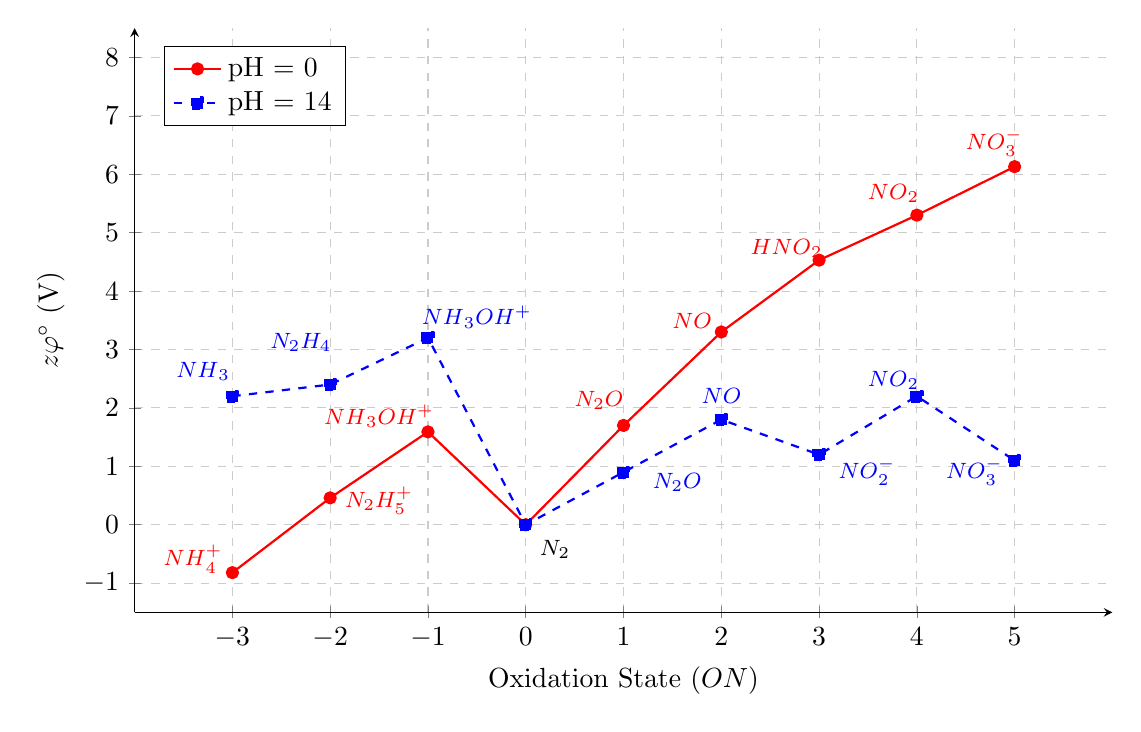
\begin{tikzpicture}
\begin{axis}[
    width=14cm,
    height=9cm,
    xlabel={Oxidation State ($ON$)},
    ylabel={$z\varphi ^\circ$ (V)},
    xmin=-4, xmax=6,
    ymin=-1.5, ymax=8.5,
    xtick={-3,-2,-1,0,1,2,3,4,5},
    ytick={-1,0,1,2,3,4,5,6,7,8},
    grid=major,
    grid style={dashed, gray!40},
    legend pos=north west,
    legend cell align={left},
    axis lines=left,
    enlargelimits=false,
    clip=false,
    every node near coord/.append style={font=\small, anchor=south west},
]

\addplot[
    color=red,
    mark=*,
    thick,
    sharp plot, 
    line join=round
] coordinates {
    (-3, -0.82)  
    (-2, 0.46)  
    (-1, 1.59) 
    (0, 0.00)  
    (1, 1.70) 
    (2, 3.3)
    (3, 4.53)
    (4, 5.3)
    (5, 6.13) 
};
\addlegendentry{pH = 0}

\node[anchor=south east, red, font=\footnotesize] at (axis cs:-3,-1) {$\text{NH}_4^+$};
\node[anchor=south, red, font=\footnotesize] at (axis cs:-1.5,0) {$\text{N}_2\text{H}_5^+$};
\node[anchor=south, red, font=\footnotesize] at (axis cs:-1.5,1.5) {$\text{NH}_3\text{OH}^+$};
\node[anchor=north, black, font=\footnotesize] at (axis cs:0.3,-0.1) {$\text{N}_2$};
\node[anchor=south west, red, font=\footnotesize] at (axis cs:0.4,1.8) {$\text{N}_2\text{O}$};
\node[anchor=south west, red, font=\footnotesize] at (axis cs:1.4,3.2) {$\text{NO}$};
\node[anchor=south west, red, font=\footnotesize] at (axis cs:2.2,4.4) {$\text{HNO}_2$};
\node[anchor=north west, red, font=\footnotesize] at (axis cs:3.4,6) {$\text{NO}_2$};
\node[anchor=south west, red, font=\footnotesize] at (axis cs:4.4,6.13) {$\text{NO}_3^-$};

\addplot[
    color=blue,
    mark=square*,
    thick,
    sharp plot, 
    dashed,
    line join=round
] coordinates {
    (-3, 2.2) 
    (-2, 2.4)  
    (-1, 3.2)  
    (0, 0.00)  
    (1, 0.9)   
    (2, 1.8)  
    (3, 1.2)  
    (4, 2.2) 
    (5, 1.1)    
};
\addlegendentry{pH = 14}
\node[anchor=south, blue, font=\footnotesize] at (axis cs:-3.3,2.3) {$\text{NH}_3$};
\node[anchor=south, blue, font=\footnotesize] at (axis cs:-2.3,2.8) {$\text{N}_2\text{H}_4$};
\node[anchor=south, blue, font=\footnotesize] at (axis cs:-0.5,3.2) {$\text{NH}_3\text{OH}^+$};
\node[anchor=south west, blue, font=\footnotesize] at (axis cs:1.2,0.4) {$\text{N}_2\text{O}$};
\node[anchor=south west, blue, font=\footnotesize] at (axis cs:1.7,1.9) {$\text{NO}$};
\node[anchor=south west, blue, font=\footnotesize] at (axis cs:3.1,0.5) {$\text{NO}_2^-$};
\node[anchor=north west, blue, font=\footnotesize] at (axis cs:3.4,2.8) {$\text{NO}_2$};
\node[anchor=south west, blue, font=\footnotesize] at (axis cs:4.2,0.5) {$\text{NO}_3^-$};

\end{axis}
\end{tikzpicture}

For example, by connecting the lines, we can see:
\begin{enumerate}
  \item Under alkaline conditions, NO and NO₂ undergo spontaneous comproportionation, while under acidic conditions, HNO₂ is unstable to disproportionation.
  \item In both acidic and alkaline media, hydroxylamine and nitrous acid (or nitrite) undergo spontaneous comproportionation to form dinitrogen.
\end{enumerate}

As emphasized in Chapter 1, this thermodynamic feasibility does not guarantee that the reaction will occur at an observable rate, as it may be limited by kinetic constraints.

\end{example}

\subsection{Effect of Conditions on Electrode Potential}

We have already established the relationship between electrode potential and Gibbs free energy. Combining this with the van’t Hoff isothermal-isobaric equation, we derive:

\begin{proposition}[Nernst Equation]
$$\varphi = \varphi^\circ - \frac{RT}{zF}\ln\frac{[\text{Red}]}{[\text{Ox}]}$$
At 298.15 K, the equation simplifies to:
$$\varphi = \varphi^\circ - \frac{0.0592}{z}\lg\frac{[\text{Red}]}{[\text{Ox}]}$$

From this equation, we see that concentration directly affects electrode potential:
\begin{enumerate}
    \item Increasing $[\text{Ox}]$ or decreasing $[\text{Red}]$ increases $\varphi$, enhancing the oxidizing power of the couple;
    \item Increasing $[\text{Red}]$ or decreasing $[\text{Ox}]$ decreases $\varphi$, enhancing the reducing power of the couple.
\end{enumerate}
This effect is more pronounced for reactions with fewer electrons transferred and at higher temperatures.
\end{proposition}

Similarly, precipitation and complexation reactions indirectly affect electrode potential by changing the effective concentration of the oxidized or reduced form:

\begin{proposition}[Effect of Precipitation and Complexation on Electrode Potential]
\begin{enumerate}
    \item Precipitation: If the oxidized form of a couple forms an insoluble precipitate, its effective concentration decreases, causing $\varphi$ to decrease (reducing oxidizing power). If the reduced form precipitates, $\varphi$ increases.
    \item Complexation: If the oxidized form forms a stable complex, its effective concentration decreases, with the same effect on $\varphi$ as precipitation.
\end{enumerate}
\end{proposition}

\begin{example}
  \begin{enumerate}
    \item As the radius of the halide ion increases (excluding fluoride, as AgF is soluble), the solubility product of the silver halide decreases. Under standard conditions (halide ion concentration = $1\ \mathrm{M}$), the $\text{Ag}^+/\text{Ag}$ electrode potential decreases, and the oxidizing power of $\text{Ag}^+$ is reduced.
    \item The principle of aqua regia dissolving gold: $\text{Au}^{3+}$ forms a stable complex $\text{AuCl}_4^-$ with $\text{Cl}^-$, which reduces $\varphi^\circ(\text{Au}^{3+}/\text{Au})$ to $\varphi^\circ(\text{AuCl}_4^-/\text{Au})$. This makes the electrode potential of the nitrate reduction couple greater than that of the gold couple, allowing the reaction to proceed spontaneously.
  \end{enumerate}
\end{example}

The Nernst equation has no explicit pH term, but for many redox couples involving oxoacids or hydroxides, the half-reaction includes $\text{H}^+$ or $\text{OH}^-$ (e.g, $\text{O}_2 + 4\text{H}^+ + 4e^- \to 2\text{H}_2\text{O}$). For these reactions, the pH of the solution has a significant effect on the electrode potential, and the Nernst equation will include a $[\text{H}^+]$ or $[\text{OH}^-]$ term. For most reduction reactions in acidic media, the electrode potential decreases as pH increases.

\begin{definition}[Pourbaix Diagram (pH-$\varphi$ Diagram)]
A Pourbaix diagram plots the electrode potential ($\varphi$) of a redox system against the pH of the solution. The diagram divides the stability regions of different chemical species and includes lines for the oxidation of water (to $\text{O}_2$) and reduction of water (to $\text{H}_2$). Species with stability regions between these two lines are thermodynamically stable in water. Due to the slow kinetics of water oxidation and reduction, the practical stability region is often extended by $\pm 0.5\ \mathrm{V}$ from the thermodynamic lines.
\end{definition}

\newpage
\begin{example}[Example of a Pourbaix Diagram]
  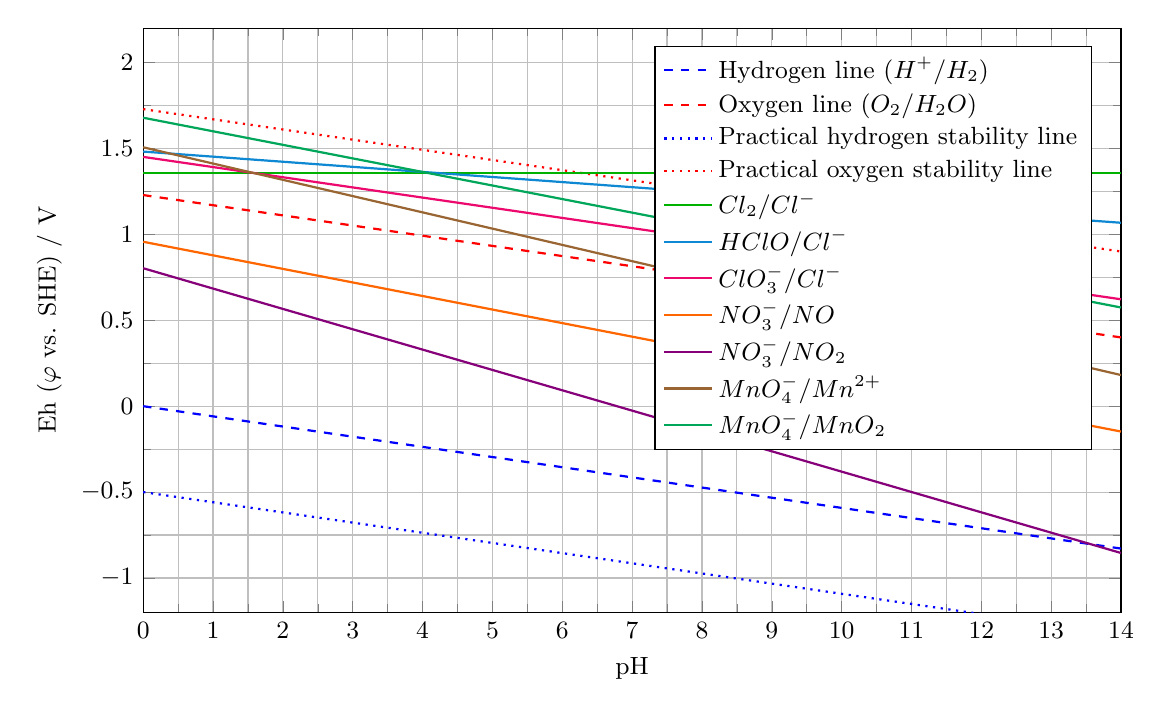
\begin{tikzpicture}
\begin{axis}[
    width=14cm,
    height=9cm,
    xlabel={pH},
    ylabel={Eh ($\varphi $ vs. SHE) / V},
    xmin=0, xmax=14,
    ymin=-1.2, ymax=2.2,
    grid=both,
    minor tick num=1,
    legend pos=north east, 
    legend style={font=\small, cells={anchor=west}},
    every axis plot/.append style={thick},
    tick label style={font=\small},
    label style={font=\small}
]

\addplot[blue, dashed, domain=0:14, samples=100] {0 - 0.0592*x};
\addplot[red, dashed, domain=0:14, samples=100] {1.229 - 0.0592*x};
\addplot[blue, dotted, domain=0:14, samples=100] {0 - 0.0592*x - 0.5};
\addplot[red, dotted, domain=0:14, samples=100] {1.229 - 0.0592*x + 0.5};

\addplot[green!70!black, domain=0:14, samples=100] {1.358};
\addplot[cyan!70!blue, domain=0:14, samples=100] {1.482 - 0.0296*x};
\addplot[magenta!70!red, domain=0:14, samples=100] {1.451 - 0.0592*x};
\addplot[orange!80!red, domain=0:14, samples=100] {0.957 - 0.0789*x};
\addplot[purple!70!blue, domain=0:14, samples=100] {0.803 - 0.1184*x};
\addplot[brown!80!black, domain=0:14, samples=100] {1.507 - 0.0947*x};
\addplot[teal!70!green, domain=0:14, samples=100] {1.679 - 0.0789*x};
\legend{
    Hydrogen line ($\text{H}^+/\text{H}_2$),
    Oxygen line ($\text{O}_2/\text{H}_2\text{O}$),
    Practical hydrogen stability line,
    Practical oxygen stability line,
    $\text{Cl}_2/\text{Cl}^-$,
    $\text{HClO}/\text{Cl}^-$,
    $\text{ClO}_3^-/\text{Cl}^-$,
    $\text{NO}_3^-/\text{NO}$,
    $\text{NO}_3^-/\text{NO}_2$,
    $\text{MnO}_4^-/\text{Mn}^{2+}$,
    $\text{MnO}_4^-/\text{MnO}_2$
}
\end{axis}
\end{tikzpicture}

In general, the electrode potential for reduction reactions involving $\text{H}^+$ decreases linearly with increasing pH, while for reactions not involving $\text{H}^+$ or $\text{OH}^-$, the plot is a horizontal line independent of pH.
\end{example}

\newpage
